\chapter{动态规划}
如果一个问题具有以下两个要素:
\begindot
\item 最优子结构(optimal substructure)
\item 重叠子问题(overlap subproblem)
\myenddot
则可以用动态规划求最优解。

动态规划分为4个步骤:
\begindot
\item 描述最优解的结构。即抽象出一个状态来表示最优解。
\item 递归的定义最优解的值。找出状态转移方程,然后递归的定义
\item 计算最优解的值。典型的做法是自底向上,当然也可以自顶向下。
\item 根据计算过程中得到的信息,构造出最优解。如果我们只需要最优解的值,不需要最
优解本身,则可以忽略第4步。当执行第4步时,我们需要在第3步的过程中维护一些额外的
信息,以便我们能方便的构造出最优解。
\myenddot
在第1步中,我们需要抽象出一个“状态”,在第2步中,我们要找出“状态转移方程”,然后才能
递归的定义最优解的值。第3步和第4步就是写代码实现了。

写代码实现时有两种方式,“递归(recursive)+自顶向下(top-down)+表格(memoization)”和
“自底向上(bottom-up)+表格”。自顶向下也称为记忆化搜索,自底向上也称为递推(不是递归)。

动规用表格将各个子问题的最优解存起来,避免重复计算,是一种空间换时间。

动规与贪心的相同点:最优子结构。

不同点:1、动规的子问题是重叠的,而贪心的子问题是不重叠的(disjoint subproblems);
2、动规不具有贪心选择性质;3、贪心的前进路线是一条线,而动规是一个DAG。

分治和贪心的相同点:disjoint subproblems。

\section{数字三角形} %%%%%%%%%%%%%%%%%%%%%%%%%%%%%

\subsubsection{描述}
有一个由非负整数组成的三角形,第一行只有一个数,除了最下一行之外每个数的左下角和右下
角各有一个数,如图~~\ref{fig:numbersTriangle}所示。

\begin{center}
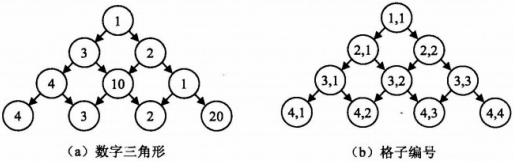
\includegraphics[width=360pt]{numbers-triangle.png}\\
\figcaption{数字三角形问题}\label{fig:numbersTriangle}
\end{center}

从第一行的数开始,每次可以往左下或右下走一格,直到走到最下行,把沿途经过的数全部加起来。
如何走才能使得这个和最大?

\subsubsection{输入}
Your program is to read from standard input. The first line contains one integer N: the 
number of rows in the triangle. The following N lines describe the data of the triangle. 
The number of rows in the triangle is > 1 but <= 100. The numbers in the triangle, 
all integers, are between 0 and 99.

\subsubsection{输出}
Your program is to write to standard output. The highest sum is written as an integer.

\subsubsection{样例输入}
\begin{Code}
5
7
3 8 
8 1 0  
2 7 4 4 
4 5 2 6 5
\end{Code}

\subsubsection{样例输出}
\begin{Code}
30
\end{Code}

\subsubsection{分析}
这是一个动态决策问题,在每层有两种选择,左下或右下,因此一个n层的数字三角形有$2^n$条路线。

可以用回溯法,用回溯法求出所有可能的路线,就可以从中选出最优路线。但是由于有$2^n$条路线,
回溯法很慢。

本题可以用动态规划来求解(具有最有子结构和重叠子问题两个要素,后面会看到)。把当前位置(i,j)看
成一个状态,然后定义状态(i,j)的指数函数d(i,j)为从位置(i,j)出发时能得到的最大和(包括格子(i,j)本
身的值a(i,j))。在这个状态定义下,原问题的解是d(1,1)。

下面来看看不同状态之间是怎样转移的。从位置(i,j)出发有两种决策,如果往左走,则走到(i+1,j)后需要求
“从(i+1,j)出发后能得到的最大和”这一子问题,即d(i+1,j),类似地,往右走之后需要求d(i+1,j+1)。应该
选择d(i+1,j)和d(i+1,j+1)中较大的一个,因此可以得到如下的状态转移方程:
$$d(i,j)=a(i,j)+\max\left\{d(i+1,j), d(i+1,j+1)\right\}$$

\subsubsection{代码}
版本1,自顶向下。

\begin{Codex}[label=numbers_triangle1.c]
#include<stdio.h>
#include<string.h>

#define MAXN 100

int n, a[MAXN][MAXN], d[MAXN][MAXN];

int max(const int x, const int y) {
    return x > y ? x : y;
}

/**
 * @brief 求从位置(i,j)出发时能得到的最大和
 * @param[in] i 行
 * @param[in] j 列
 * @return 最大和
 */
int dp(const int i, const int j) {
    if(d[i][j] >= 0) {
        return d[i][j];
    } else {
        return d[i][j] = a[i][j] + (i == n-1 ? 0 : max(dp(i+1, j+1), dp(i+1, j)));
    }
}

int main() {
    int i, j;
    memset(d, -1, sizeof(d));

    scanf("%d", &n);
    for(i = 0; i < n; i++)
      for (j = 0; j <= i; j++) scanf("%d", &a[i][j]);
    
    printf("%d\n", dp(0, 0));
    return 0;
}
\end{Codex}

版本2,自底向上。

\begin{Codex}[label=numbers_triangle2.c]
#include<stdio.h>
#include<string.h>

#define MAXN 100

int n, a[MAXN][MAXN], d[MAXN][MAXN];

int max(const int x, const int y) {
    return x > y ? x : y;
}

/**
 * @brief 自底向上计算所有子问题的最优解
 * @return 无
 */
void dp() {
    int i, j;
    for (i = 0; i < n; ++i) {
        d[n-1][i] = a[n-1][i];
    }
    for (i = n-2; i >= 0; --i)
      for (j = 0; j <= i; ++j)
        d[i][j] = a[i][j] + max(d[i+1][j], d[i+1][j+1]);
}

int main() {
    int i, j;
    memset(d, -1, sizeof(d));

    scanf("%d", &n);
    for(i = 0; i < n; i++)
      for (j = 0; j <= i; j++) 
          scanf("%d", &a[i][j]);

    dp();
    
    printf("%d\n", d[0][0]);
    return 0;
}
\end{Codex}

\subsubsection{类似的题目}
与本题相同的题目:
\begindot
\item 《算法竞赛入门经典》\footnote{刘汝佳,算法竞赛入门经典,清华大学出版社,2009}第159页9.1.1节
\item  POJ 1163 - The Triangle, \myurl{http://poj.org/problem?id=1163}
\myenddot

与本题相似的题目:
\begindot
\item  TODO
\myenddot

\section{DAG上的动态规划} %%%%%%%%%%%%%%%%%%%%%%%%%%%%%%

\subsection{嵌套矩形}

\subsubsection{描述}
有$n$个矩形,每个矩形可以用$a,b$来描述,表示长和宽。矩形$X(a,b)$可以嵌套在
矩形$Y(c,d)$中当且仅当$a<c,b<d$或者$b<c,a<d$(相当于旋转X90度)。例如
(1,5)可以嵌套在(6,2)内,但不能嵌套在(3,4)中。你的任务是选出尽可能多的
矩形排成一行,使得除最后一个外,每一个矩形都可以嵌套在下一个矩形内。

\subsubsection{输入}
第一行是一个正正数$N(0<N<10)$,表示测试数据组数,
每组测试数据的第一行是一个正正数n,表示该组测试数据中含有矩形的个数$(n<=1000)$
随后的n行,每行有两个数$a,b(0<a,b<100)$,表示矩形的长和宽

\subsubsection{输出}
每组测试数据都输出一个数,表示最多符合条件的矩形数目,每组输出占一行

\subsubsection{样例输入}
\begin{Code}
1
10
1 2
2 4
5 8
6 10
7 9
3 1
5 8
12 10
9 7
2 2
\end{Code}

\subsubsection{样例输出}
\begin{Code}
5
\end{Code}

\subsubsection{分析}
本题实质上是求DAG中不固定起点的最长路径。

设d[i]表示从结点i出发的最长长度,状态转移方程如下:
$$d[i]=\max\left\{d[j]+1|(i,j) \in E\right\}$$

其中,E为边的集合。最终答案是d[i]中的最大值。

\subsubsection{代码}
\begin{Codex}[label=embedded_rectangles.c]
#include <stdio.h>
#include <string.h>

#define MAXN 1000 // 矩形最大个数

int n; // 矩形个数
int G[MAXN][MAXN]; // 矩形包含关系
int d[MAXN]; // 表格

/**
 * @brief 动规,自顶向下.
 * @param[in] i 起点
 * @return 以i为起点,能达到的最长路径
 */
int dp(const int i) {
    int j;
    int *ans= &d[i];
    if(*ans > 0) return *ans;

    *ans = 1;
    for(j = 0; j < n; j++) if(G[i][j]) {
        const int next = dp(j) + 1;
        if(*ans < next) *ans = next;
    }
    return *ans;
}

/**
 * @brief 按字典序打印路径.
 *
 * 如果多个 d[i] 相等,选择最小的i。
 *
 * @param[in] i 起点
 * @return 无
 */
void print_path(const int i) {
    int j;
    printf("%d ", i);
    for(j = 0; j < n; j++) if(G[i][j] && d[i] == d[j] + 1) {
        print_path(j);
        break;
    }
}

int main() {
    int N, i, j;
    int max, maxi;
    int a[MAXN],b[MAXN];

    scanf("%d", &N);
    while(N--) {
        memset(G, 0, sizeof(G));
        memset(d, 0, sizeof(d));

        scanf("%d", &n);
        for(i = 0; i < n; i++) scanf("%d%d", &a[i], &b[i]);

        for(i = 0; i < n; i++)
            for(j = 0; j < n; j++)
                if((a[i] > a[j] && b[i] > b[j]) ||
                    (a[i] > b[j] && b[i] > a[j])) G[i][j] = 1;

        max = 0;
        maxi = -1;
        for(i = 0; i < n; i++) if(dp(i) > max) {
            max = dp(i);
            maxi = i;
        }
        printf("%d\n", max);
        // print_path(maxi);
    }
    return 0;
}
\end{Codex}

\subsubsection{类似的题目}
与本题相同的题目:
\begindot
\item 《算法竞赛入门经典》\footnote{刘汝佳,算法竞赛入门经典,清华大学出版社,2009}第161页9.2.1节
\item  NYOJ 16 嵌套矩形, \myurl{http://acm.nyist.net/JudgeOnline/problem.php?pid=16}
\myenddot

与本题相似的题目:
\begindot
\item  TODO
\myenddot

\subsection{硬币问题}

\subsubsection{描述}
有$n$种硬币,面值为别为$v_1,v_2,v_3,\cdots, v_n$,每种都有无限多。给定非负整数$S$,可以
选取多少个硬币,使得面值和恰好为$S$?输出硬币数目的最小值和最大值。$1 \leq n \leq 100, 1 \leq S \leq 10000, 1 \leq v_i \leq S$。

\subsubsection{输入}
第1行$n$,
第2行$S$,
第3到$n+2$行为$n$种不同的面值。

\subsubsection{输出}
第1行为最小值,
第2行为最大值。

\subsubsection{分析}
本题实质上是求DAG中固定终点的最长路径和最短路径。

\subsubsection{代码}
版本1,自顶向下。

\begin{Codex}[label=coin_change.c]
#include<stdio.h>
#include <string.h>

#define MAXN 100
#define MAXV 10000

/** 硬币面值的种类. */
int n;
/** 要找零的数目. */
int S;
/** 硬币的各种面值. */
int v[MAXN];
/** min[i] 表示面值之和为i的最短路径的长度,max则是最长. */
int min[MAXV + 1], max[MAXV + 1];

/**
 * @brief 最短路径.
 * @param[in] s 面值
 * @return 最短路径长度
 */
int dp1(const int s) { // 最小值
    int i;
    int *ans = &min[s];
    if(*ans != -1) return *ans;
    *ans = 1<<30;
    for(i = 0; i < n; ++i) if(v[i] <= s) {
        const int tmp = dp1(s-v[i])+1;
        *ans = *ans < tmp ? *ans : tmp;
    }
    return *ans;
}

int visited[MAXV + 1];
/**
 * @brief 最长路径.
 * @param[in] s 面值
 * @return 最长路径长度
 */
int dp2(const int s) { //最大值 
    int i;
    int *ans = &max[s];

    if(visited[s]) return max[s];
    visited[s] = 1;

    *ans = -1<<30;
    for(i = 0; i < n; ++i) if(v[i] <= s) {
        const int tmp = dp2(s-v[i])+1;
        *ans = *ans > tmp ? *ans : tmp;
    }
    return *ans;
}

/**
 * @brief 打印路径.
 * @param[in] d 上面的 min 或 min
 * @param[in] s 面值之和
 * @return 无
 */
void print_path(const int* d, const int s){//打印的是边
    int i;
    for(i = 0; i < n; ++i) if(v[i] <= s && d[s-v[i]] + 1 == d[s]) {
        printf("%d ",i);
        print_path(d, s-v[i]);
        break;
    }
    printf("\n");
}

int main() {
    int i;
    scanf("%d%d", &n, &S);
    for(i = 0; i < n; ++i) scanf("%d", &v[i]);

    memset(min, -1, sizeof(min));
    min[0] = 0;
    printf("%d\n", dp1(S));
    // print_path(min, S);

    memset(max, -1, sizeof(max));
    memset(visited, 0, sizeof(visited));
    max[0] = 0; visited[0] = 1;
    printf("%d\n", dp2(S));
    // print_path(max, S);

    return 0;
}
\end{Codex}

版本2,自底向上。

\begin{Codex}[label=coin_change2.c]
#include<stdio.h>

#define MAXN 100
#define MAXV 10000

int n, S, v[MAXN], min[MAXV + 1], max[MAXV + 1];
int min_path[MAXV], max_path[MAXV];
/**
 * @brief 打印路径.
 * @param[in] d 上面的 min_path 或 min_path
 * @param[in] s 面值之和
 * @return 无
 */
void print_path(const int *d, int s) {
    while(s) {
        printf("%d ", d[S]);
        S -= v[d[s]];
    }
    printf("\n");
}

int main() {
    int i, j;
    scanf("%d%d", &n, &S);
    for(i = 0; i < n; ++i) scanf("%d", &v[i]);

    min[0] = max[0] = 0;
    for(i = 1; i <= S; ++i) {
        min[i] = MAXV; 
        max[i] = -MAXV;
    }

    for(i = 1; i <= S; ++i) {
        for(j = 0; j < n; ++j) if(v[j] <= i) {
            if(min[i-v[j]] + 1 < min[i]) {
                min[i] = min[i-v[j]] + 1;
                min_path[i] = j;
            }
            if(max[i-v[j]] + 1 > max[i]) {
                max[i] = max[i-v[j]] + 1;
                max_path[i] = j;
            }
        }
    }
    printf("%d\n", min[S]);
    // print_path(min_path, S);
    printf("%d\n", max[S]);
    // print_path(max_path, S);
    return 0;
}
\end{Codex}

\subsubsection{类似的题目}
与本题相同的题目:
\begindot
\item 《算法竞赛入门经典》\footnote{刘汝佳,算法竞赛入门经典,清华大学出版社,2009}第162页例题9-3
\item  tyvj 1214 硬币问题, \myurl{http://www.tyvj.cn/problem_show.aspx?id=1214}
\myenddot

与本题相似的题目:
\begindot
\item  TODO
\myenddot

\section{背包问题} %%%%%%%%%%%%%%%%%%%%%%%%%%%%%%
背包问题(Knapsack problem\footnote{Knapsack problem, \myurl{http://en.wikipedia.org/wiki/Knapsack_problem}})有很多种版本,
常见的是以下三种:
\begindot
\item 0-1背包问题(0-1 knapsack problem):每种物品只有一个
\item 完全背包问题(UKP, unbounded knapsack problem):每种物品都有无限个可用
\item 多重背包问题(BKP, bounded knapsack problem):第i种物品有c[i]个可用
\myenddot

其他版本的背包问题请参考“背包问题九讲”,\myurl{https://github.com/tianyicui/pack}

\subsection{0-1背包问题}

\subsubsection{描述}
有$n$种物品,第$i$种物品的重量为$w_i$,价值为$v_i$,每种物品只有一个。背包能承受的重量为$W$。
将哪些物品装入背包可使这些物品的总重量不超过背包容量,且价值总和最大?

\subsubsection{输入}
第1行包含一个整数T,是案例的个数。
接下来是T个案例,每个案例3行,第1行包含两个整数$n, W(n \leq 1000 , W \leq 1000)$分别表示
物品的种数和背包的容量,第2行包含n个整数表示每种物品的价值,第3行包含n个整数表示每种物品的重量。

\subsubsection{输出}
每行一个整数,表示价值总和的最大值。

\subsubsection{样例输入}
\begin{Code}
1
5 10
1 2 3 4 5
5 4 3 2 1
\end{Code}

\subsubsection{样例输出}
\begin{Code}
14
\end{Code}

\subsubsection{分析}
由于每种物品仅有一个,可以选择装或者不装。

定义状态f[i][j],表示“把前i个物品装进容量为j的背包可以获得的最大价值”,
则其状态转移方程便是:
$$f[i][j]=\max\left\{f[i-1][j], f[i-1][j-w[i]+v[i]\right\}$$

这个方程理解如下,把前i个物品装进容量为j的背包时,有两种情况:
\begindot
\item 第i个不装进去,这时所得价值为:$f[i-1][j]$
\item 第i个装进去,这时所得价值为:$f[i-1][j-w[i]+v[i]$
\myenddot

动规过程的伪代码如下:
\begin{Code}
for i=1..n
    for j=0..W
        f[j]=max{f[j],f[j-w[i]]+v[i]};
\end{Code}

内循环从右向左也可以:
\begin{Code}
for i=1..n
    for j=W..0
        f[j]=max{f[j],f[j-w[i]]+v[i]};
\end{Code}

内循环从右向左时,可以把二维数组优化成一维数组。为什么呢?举个例子,测试数据如下:
\begin{Code}
1
3 10
4 5 6
3 4 5
\end{Code}

f是从上到下、从右到左计算的,如图~\ref{fig:01pack}所示。
\begin{center}
\includegraphics[width=360pt]{01pack.gif}\\
\figcaption{0-1背包问题的计算顺序}\label{fig:01pack}
\end{center}

当内循环是逆序时,且动规是用自底向上方式实现时,就可以保证同一行可以从右向左更新。

设一维数组为d(又称为滚动数组\footnote{刘汝佳,算法竞赛入门经典,清华大学出版社,2009,第169页9.3.3节}),
在更新d[j]之前,d[j]里保存的f[i-1][j],更新之后,d[j]里保存的是f[i][j]。

\subsubsection{代码}
版本1,自底向上。

\begin{Codex}[label=01knapsack.c]
#include <stdio.h>
#include <string.h>

#define MAXN 1000
#define MAXW 1000

int T;
int n, W;
int w[MAXN+1], v[MAXN+1]; /* 0 没有用 */

int f[MAXN + 1][MAXW + 1];

int main() {
    scanf("%d", &T);
    while(T--) {
        int i, j;
        memset(f, 0, sizeof(f));
        scanf("%d %d", &n, &W);
        for(i = 1; i <= n; ++i) scanf("%d", &v[i]);
        for(i = 1; i <= n; ++i) scanf("%d", &w[i]);

        for(i = 1; i <= n; ++i) {
            /* for(j = W; j >= 0; --j) { /* 也可以 */
            for(j = 0; j <= W; ++j) {
                f[i][j] = f[i-1][j];
                if(j >= w[i]) {
                    const int tmp = f[i-1][j-w[i]] + v[i];
                    if(tmp > f[i][j]) f[i][j] = tmp;
                }
            }
        }
        printf("%d\n", f[n][W]);
    }
    return 0;
}
\end{Codex}

版本2,自底向上,滚动数组。

\begin{Codex}[label=01knapsack2.c]
#include <stdio.h>
#include <string.h>

#define MAXN 1000
#define MAXW 1000

int T;
int n, W;
int w[MAXN], v[MAXN];

int d[MAXW + 1]; /* 滚动数组 */

int main() {
    scanf("%d", &T);
    while(T--) {
        int i, j;
        memset(d, 0, sizeof(d));
        scanf("%d %d", &n, &W);
        for(i = 0; i < n; ++i) scanf("%d", &v[i]);
        for(i = 0; i < n; ++i) scanf("%d", &w[i]);

        for(i = 0; i < n; ++i) {
            for(j = W; j >= w[i]; --j) {
                const int tmp = d[j - w[i]] + v[i];
                if(tmp > d[j]) d[j] = tmp;
            }
        }
        printf("%d\n", d[W]);
    }
    return 0;
}
\end{Codex}

\subsubsection{类似的题目}
与本题相同的题目:
\begindot
\item 《算法竞赛入门经典》\footnote{刘汝佳,算法竞赛入门经典,清华大学出版社,2009}第167页例题9-5
\item  HDOJ 2602 Bone Collector, \myurl{http://acm.hdu.edu.cn/showproblem.php?pid=2602}
\myenddot

与本题相似的题目:
\begindot
\item  TODO
\myenddot

\subsection{完全背包问题}

\subsubsection{描述}
每种物品有无限个可用,其他信息与0-1背包相同。

\subsubsection{分析}
状态转移方程为:
$$f[i][j]=\max\left\{f[i-1][j-k*w[i]+k*v[i], 0 \leq k*w[i] \leq j\right\}$$

\subsubsection{代码}
\begin{Codex}[label=ukp.c]

\end{Codex}

\subsection{多重背包问题}

\subsubsection{描述}
第i种物品有c[i]个可用,其他信息与0-1背包相同。

\subsubsection{分析}
状态转移方程为:
$$f[i][j]=\max\left\{f[i-1][j-k*w[i]+k*v[i], 0 \leq k*w[i] \leq j, 0 \leq k \leq c[i]\right\}$$

\subsubsection{代码}
\begin{Codex}[label=bkp.c]

\end{Codex}

\section{最长公共子序列} %%%%%%%%%%%%%%%%%%%%%%%%%%%%%%